% GeoMind: Complete Experimental Results (appendix body)
% \graphicspath{{paper/figures/}{figures/}} recommended (see appendix_results_dashboard_preamble.tex)

\section{Complete Experimental Results}
\label{app:complete_results}

This appendix provides a consolidated dashboard of GeoMind results intended for benchmark transparency. Family-level aggregates summarize broad trends, while task-level tables expose variation that is often hidden by averages. Diagnostic metrics complement binary success rates by characterizing spatial goal error, trajectory-level execution error, and dominant failure modes. Throughout, values are reported as success rates (\%) unless stated otherwise.

%--------------------------------------------------------------------
\subsection{Result Dashboard}
\label{app:subsec:dashboard}

Figure~\ref{fig:app_result_dashboard} summarizes overall performance on GeoMind-Base and GeoMind-Aug, contrasts methods grouped by implementation paradigm, and visualizes average robustness under semantic, visual, and execution augmentations. The dashboard is designed to make oracle gaps, cross-paradigm differences, and augmentation-induced degradation immediately visible to reviewers.

\begin{figure*}[t]
  \centering
  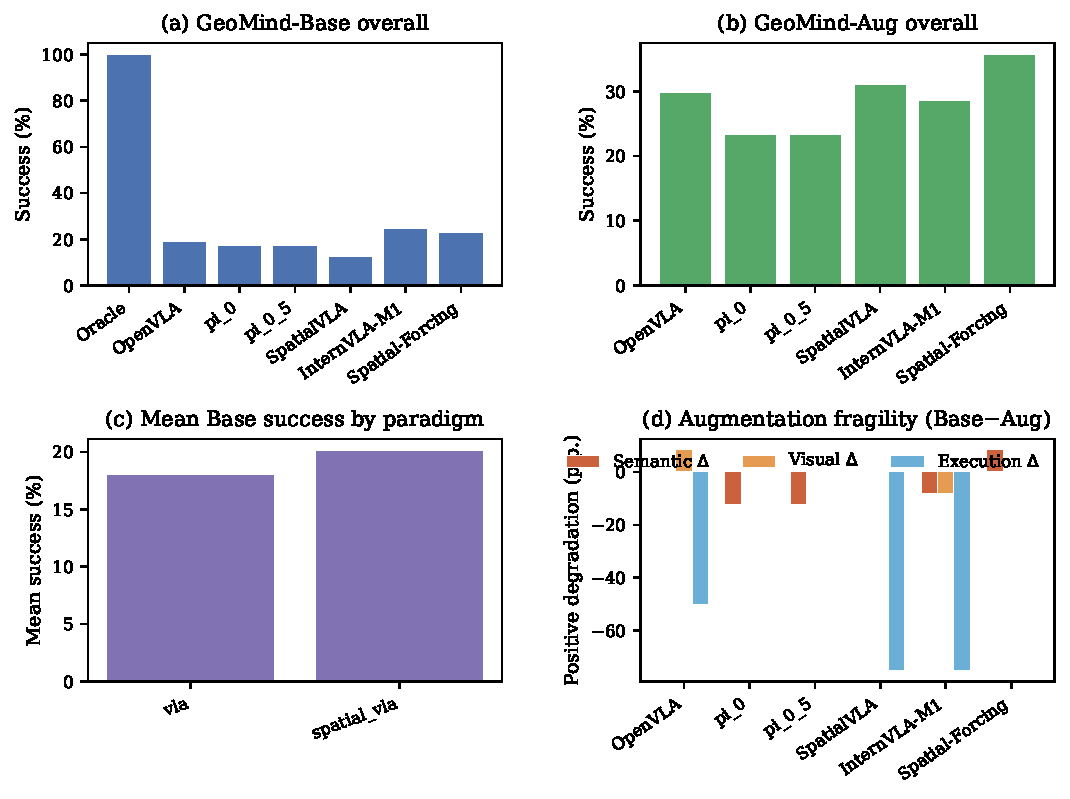
\includegraphics[width=\linewidth]{figures/app_result_dashboard.pdf}
  \caption{\textbf{Appendix result dashboard.} (a)~Overall success on GeoMind-Base. (b)~Overall success on GeoMind-Aug. (c)~Average success by method paradigm (VLA, spatial-enhanced VLA, modular). (d)~Average performance drop under semantic, visual, and execution augmentations, where each bar reports positive degradation as $\Delta = \text{Base}-\text{Aug}$ in percentage points for the matched task set (higher indicates greater fragility). Base and Aug panels report success rates (\%). Augmentation changes in Table~\ref{tab:app_aug_complete} use percentage-point shifts $\text{Aug}-\text{Base}$ for each augmentation column. The gap to the oracle highlights that many tasks are physically feasible under full information yet remain challenging for current agents.}
  \label{fig:app_result_dashboard}
\end{figure*}

%--------------------------------------------------------------------
\subsection{Complete Results on GeoMind-Base}
\label{app:subsec:base}

Table~\ref{tab:app_base_complete} reports complete success rates on GeoMind-Base across six task families, together with aggregated \emph{Spatial Reasoning} and \emph{Spatial Memory} averages and an overall mean. The complete results support the main-paper observation that performance is uneven across families, and the gap to the oracle suggests that failures are not uniformly explained by low-level control noise alone.

\begin{table*}[t]
  \centering
  \small
  \setlength{\tabcolsep}{4pt}
  \resizebox{\textwidth}{!}{%
  \begin{tabular}{lccccccccc}
    \toprule
    \rowcolor{HeaderGray}
    Method
      & \makecell{Target\\Ident.}
      & \makecell{Relational\\Grounding}
      & \makecell{Constraint\\Composition}
      & \makecell{Geometric\\Inference}
      & \makecell{Scene\\Updating}
      & \makecell{Identity\\Tracking}
      & \makecell{\textbf{Spat.~Reas.}\\\textbf{Avg.}}
      & \makecell{\textbf{Spat.~Mem.}\\\textbf{Avg.}}
      & \makecell{\textbf{Overall}\\\textbf{Avg.}} \\
    \midrule
        \rowcolor{OracleFill}
    Oracle
      & 100.0 & 100.0 & 100.0 & 100.0 & 100.0 & 100.0 & \textbf{100.0} & \textbf{100.0} & \textbf{100.0} \\
    \midrule
    \rowcolor{VLAFill}
    OpenVLA
      & 37.5 & 0.0 & 6.2 & 5.0 & 41.7 & 25.0 & \textbf{12.2} & \textbf{33.3} & \textbf{19.2} \\
    \rowcolor{VLAFill}
    $\pi_0$
      & 9.4 & 0.0 & 40.6 & 0.0 & 35.4 & 18.8 & \textbf{12.5} & \textbf{27.1} & \textbf{17.4} \\
    \rowcolor{VLAFill}
    $\pi_{0.5}$
      & 9.4 & 0.0 & 40.6 & 0.0 & 35.4 & 18.8 & \textbf{12.5} & \textbf{27.1} & \textbf{17.4} \\
    \midrule
    \rowcolor{SpatialVLAFill}
    SpatialVLA
      & 0.0 & 4.2 & 0.0 & 17.5 & 45.8 & 8.3 & \textbf{5.4} & \textbf{27.1} & \textbf{12.6} \\
    \rowcolor{SpatialVLAFill}
    InternVLA-M1
      & 42.5 & 50.0 & 6.2 & 12.0 & 16.7 & 20.8 & \textbf{27.7} & \textbf{18.8} & \textbf{24.7} \\
    \rowcolor{SpatialVLAFill}
    Spatial-Forcing
      & 12.5 & 0.0 & 50.0 & 5.0 & 33.3 & 37.5 & \textbf{16.9} & \textbf{35.4} & \textbf{23.1} \\
    \midrule
    \rowcolor{ModularFill}
    COPA-GPT-4o
      & \textemdash{} & \textemdash{} & \textemdash{} & \textemdash{} & \textemdash{} & \textemdash{} & \textbf{\textemdash{}} & \textbf{\textemdash{}} & \textbf{\textemdash{}} \\
    \rowcolor{ModularFill}
    COPA-Gemini
      & \textemdash{} & \textemdash{} & \textemdash{} & \textemdash{} & \textemdash{} & \textemdash{} & \textbf{\textemdash{}} & \textbf{\textemdash{}} & \textbf{\textemdash{}} \\
    \rowcolor{ModularFill}
    COPA-Claude
      & \textemdash{} & \textemdash{} & \textemdash{} & \textemdash{} & \textemdash{} & \textemdash{} & \textbf{\textemdash{}} & \textbf{\textemdash{}} & \textbf{\textemdash{}} \\
    \rowcolor{ModularFill}
    MOKA-GPT-4o
      & \textemdash{} & \textemdash{} & \textemdash{} & \textemdash{} & \textemdash{} & \textemdash{} & \textbf{\textemdash{}} & \textbf{\textemdash{}} & \textbf{\textemdash{}} \\
    \rowcolor{ModularFill}
    MOKA-Gemini
      & \textemdash{} & \textemdash{} & \textemdash{} & \textemdash{} & \textemdash{} & \textemdash{} & \textbf{\textemdash{}} & \textbf{\textemdash{}} & \textbf{\textemdash{}} \\
    \rowcolor{ModularFill}
    MOKA-Claude
      & \textemdash{} & \textemdash{} & \textemdash{} & \textemdash{} & \textemdash{} & \textemdash{} & \textbf{\textemdash{}} & \textbf{\textemdash{}} & \textbf{\textemdash{}} \\

    \bottomrule
  \end{tabular}%
  }
  \caption{\textbf{Complete success rates on GeoMind-Base.} Values are percentages. \emph{Spatial Reasoning Avg.} aggregates Target Identification, Relational Grounding, Constraint Composition, and Geometric Inference. \emph{Spatial Memory Avg.} aggregates Scene Updating and Identity Tracking. Shading indicates method families (oracle, VLA policies, spatial-enhanced VLA policies, modular agents). Numeric rows are regenerated from \texttt{run\_eval\_*} summaries via \texttt{scripts/export\_paper\_appendix\_data.py}; the Oracle row uses a nominal 100\% ceiling unless a measured oracle export is provided. COPA/MOKA cells show \textemdash{} when no modular-agent runs are present under \texttt{run\_eval\_*}.}
  \label{tab:app_base_complete}
\end{table*}

The heatmap in Figure~\ref{fig:app_base_heatmap} provides an alternative visualization of the same family-level matrix, emphasizing relative strengths and weaknesses across methods.

\begin{figure*}[t]
  \centering
  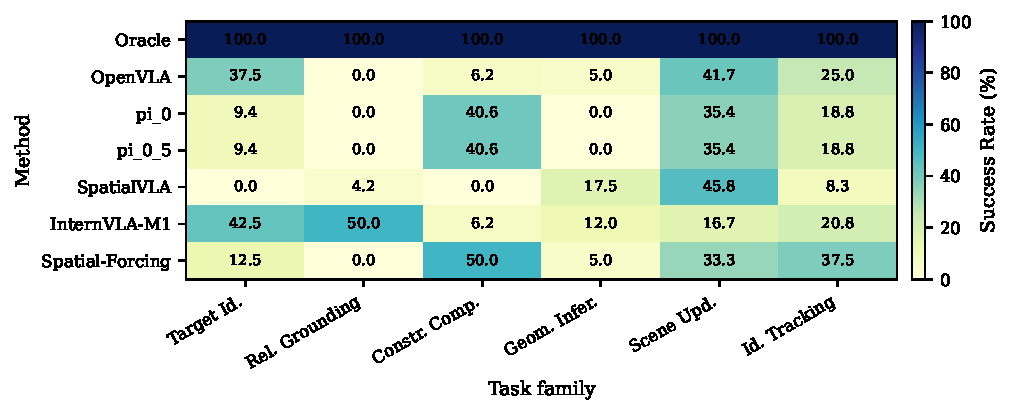
\includegraphics[width=0.92\linewidth]{figures/app_base_heatmap.pdf}
  \caption{\textbf{GeoMind-Base family-level success heatmap.} Rows correspond to methods and columns to task families. Cell entries show success rates (\%). Darker colors indicate higher success under the chosen colormap; the color scale is aligned across methods to support cross-row comparison.}
  \label{fig:app_base_heatmap}
\end{figure*}

%--------------------------------------------------------------------
\subsection{Complete Results on GeoMind-Aug}
\label{app:subsec:aug}

Table~\ref{tab:app_aug_complete} reports GeoMind-Aug performance under semantic, visual, and execution perturbations. Each augmentation cell uses the format ``success (drop)'', where drop is the percentage-point change relative to the corresponding Base tasks, $\text{Aug}-\text{Base}$. The augmentation results show that some Base successes are fragile under controlled semantic, visual, or execution changes.

\textit{Clarification.} Here \emph{Base Avg.} is aligned with the six-family mean in Table~\ref{tab:app_base_complete} (same \texttt{family\_by\_model\_long} aggregation). Augmentation columns use strict-tier paired tasks from the run matrix; \emph{Aug Avg.} uses diagnostics suite aggregates when available, otherwise the mean of the semantic, visual, and execution cells above.

\begin{table*}[t]
  \centering
  \small
  \setlength{\tabcolsep}{5pt}
  \resizebox{\textwidth}{!}{%
  \begin{tabular}{lcccccc}
    \toprule
    \rowcolor{HeaderGray}
    Method
      & Base Avg.
      & Semantic
      & Visual
      & Execution
      & Aug Avg.
      & Worst Drop \\
    \midrule
        \rowcolor{VLAFill}
    OpenVLA
      & 19.2 & \augcell{25.0}{+0.0} & \augcell{16.7}{-8.3} & \augcell{50.0}{+50.0} & 29.8 & \cellcolor{DropLight}-8.3 \\
    \rowcolor{VLAFill}
    $\pi_0$
      & 17.4 & \augcell{37.5}{+12.5} & \augcell{25.0}{+0.0} & \textemdash{} & 23.3 & \cellcolor{DropLight}+0.0 \\
    \rowcolor{VLAFill}
    $\pi_{0.5}$
      & 17.4 & \augcell{37.5}{+12.5} & \augcell{25.0}{+0.0} & \textemdash{} & 23.3 & \cellcolor{DropLight}+0.0 \\
    \midrule
    \rowcolor{SpatialVLAFill}
    SpatialVLA
      & 12.6 & \augcell{16.7}{+0.0} & \augcell{16.7}{+0.0} & \augcell{75.0}{+75.0} & 31.0 & \cellcolor{DropLight}+0.0 \\
    \rowcolor{SpatialVLAFill}
    InternVLA-M1
      & 24.7 & \augcell{8.3}{+8.3} & \augcell{8.3}{+8.3} & \augcell{75.0}{+75.0} & 28.6 & \cellcolor{DropLight}+8.3 \\
    \rowcolor{SpatialVLAFill}
    Spatial-Forcing
      & 23.1 & \augcell{33.3}{-8.3} & \augcell{41.7}{+0.0} & \augcell{0.0}{+0.0} & 35.7 & \cellcolor{DropLight}-8.3 \\
    \midrule
    \rowcolor{ModularFill}
    COPA-GPT-4o
      & \textemdash{} & \textemdash{} & \textemdash{} & \textemdash{} & \textemdash{} & \cellcolor{DropLight}\textemdash{} \\
    \rowcolor{ModularFill}
    COPA-Gemini
      & \textemdash{} & \textemdash{} & \textemdash{} & \textemdash{} & \textemdash{} & \cellcolor{DropLight}\textemdash{} \\
    \rowcolor{ModularFill}
    COPA-Claude
      & \textemdash{} & \textemdash{} & \textemdash{} & \textemdash{} & \textemdash{} & \cellcolor{DropLight}\textemdash{} \\
    \rowcolor{ModularFill}
    MOKA-GPT-4o
      & \textemdash{} & \textemdash{} & \textemdash{} & \textemdash{} & \textemdash{} & \cellcolor{DropLight}\textemdash{} \\
    \rowcolor{ModularFill}
    MOKA-Gemini
      & \textemdash{} & \textemdash{} & \textemdash{} & \textemdash{} & \textemdash{} & \cellcolor{DropLight}\textemdash{} \\
    \rowcolor{ModularFill}
    MOKA-Claude
      & \textemdash{} & \textemdash{} & \textemdash{} & \textemdash{} & \textemdash{} & \cellcolor{DropLight}\textemdash{} \\

    \bottomrule
  \end{tabular}%
  }
  \caption{\textbf{Complete results on GeoMind-Aug.} Success rates are percentages. Numbers in parentheses denote percentage-point changes relative to the corresponding Base tasks, computed as $\text{Aug}-\text{Base}$ for each augmentation column. \emph{Worst Drop} reports the minimum (most negative) change across semantic, visual, and execution splits. Semantic, visual, and execution cells are derived from strict-tier paired columns in \texttt{run\_eval\_models\_task\_level\_matrix.csv} (see \texttt{scripts/export\_paper\_appendix\_data.py}). Figure~\ref{fig:app_aug_drop_bar} reports positive degradation $\Delta=\text{Base}-\text{Aug}$ for the same matched task sets.}
  \label{tab:app_aug_complete}
\end{table*}

\begin{figure*}[t]
  \centering
  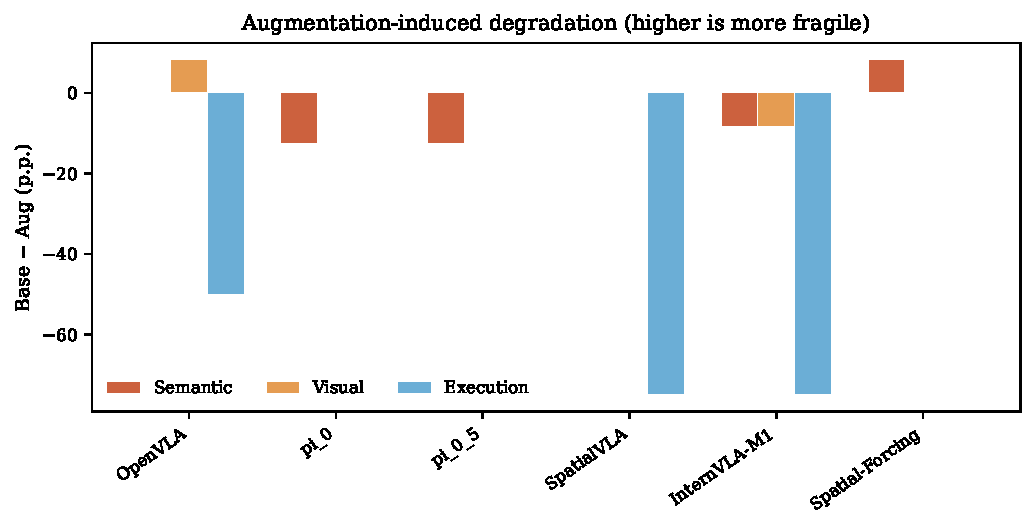
\includegraphics[width=0.85\linewidth]{figures/app_aug_drop_bar.pdf}
  \caption{\textbf{Augmentation robustness (positive degradation).} For each method, grouped bars report $\Delta=\text{Base}-\text{Aug}$ in percentage points for semantic, visual, and execution augmentations on the matched task set. Higher bars indicate greater sensitivity to controlled perturbations. This visualization complements Table~\ref{tab:app_aug_complete}, where parentheses instead report $\text{Aug}-\text{Base}$.}
  \label{fig:app_aug_drop_bar}
\end{figure*}

%--------------------------------------------------------------------
\subsection{Task-Level Results}
\label{app:subsec:tasklevel}

The task-level breakdown reveals substantial variation hidden by family-level averages. Tables~\ref{tab:app_task_tid_compact}--\ref{tab:app_task_track_compact} provide compact summaries per family for benchmark transparency; they are not intended to restate the paper's primary claims. When full per-model numbers are available, Table~\ref{tab:app_task_full} (longtable) can replace or augment the compact view.

\subsubsection{Target Identification}
\begin{table}[t]
  \centering
  \footnotesize
  \begin{tabularx}{\columnwidth}{p{0.14\linewidth} p{0.10\linewidth} X c c c c}
    \toprule
    \rowcolor{HeaderGray}
    Task ID & Struct. & Instr. Summary & Orcl. & Best VLA & Best Mod. & Best \\
    \midrule
    \TODO{} & \TODO{} & \TODO{} & \TODO{} & \TODO{} & \TODO{} & \TODO{} \\
    \TODO{} & \TODO{} & \TODO{} & \TODO{} & \TODO{} & \TODO{} & \TODO{} \\
    \bottomrule
  \end{tabularx}
  \caption{\textbf{Task-level summary (Target Identification).} Columns report oracle success, the best-performing VLA policy, the best-performing modular agent, and the best non-oracle method. Instruction summaries are abbreviated for space.}
  \label{tab:app_task_tid_compact}
\end{table}

\subsubsection{Relational Grounding}
\begin{table}[t]
  \centering
  \footnotesize
  \begin{tabularx}{\columnwidth}{p{0.14\linewidth} p{0.10\linewidth} X c c c c}
    \toprule
    \rowcolor{HeaderGray}
    Task ID & Struct. & Instr. Summary & Orcl. & Best VLA & Best Mod. & Best \\
    \midrule
    \TODO{} & \TODO{} & \TODO{} & \TODO{} & \TODO{} & \TODO{} & \TODO{} \\
    \bottomrule
  \end{tabularx}
  \caption{\textbf{Task-level summary (Relational Grounding).}}
  \label{tab:app_task_rg_compact}
\end{table}

\subsubsection{Constraint Composition}
\begin{table}[t]
  \centering
  \footnotesize
  \begin{tabularx}{\columnwidth}{p{0.14\linewidth} p{0.10\linewidth} X c c c c}
    \toprule
    \rowcolor{HeaderGray}
    Task ID & Struct. & Instr. Summary & Orcl. & Best VLA & Best Mod. & Best \\
    \midrule
    \TODO{} & \TODO{} & \TODO{} & \TODO{} & \TODO{} & \TODO{} & \TODO{} \\
    \bottomrule
  \end{tabularx}
  \caption{\textbf{Task-level summary (Constraint Composition).}}
  \label{tab:app_task_cc_compact}
\end{table}

\subsubsection{Geometric Inference}
\begin{table}[t]
  \centering
  \footnotesize
  \begin{tabularx}{\columnwidth}{p{0.14\linewidth} p{0.10\linewidth} X c c c c}
    \toprule
    \rowcolor{HeaderGray}
    Task ID & Struct. & Instr. Summary & Orcl. & Best VLA & Best Mod. & Best \\
    \midrule
    \TODO{} & \TODO{} & \TODO{} & \TODO{} & \TODO{} & \TODO{} & \TODO{} \\
    \bottomrule
  \end{tabularx}
  \caption{\textbf{Task-level summary (Geometric Inference).}}
  \label{tab:app_task_geo_compact}
\end{table}

\subsubsection{Scene Updating}
\begin{table}[t]
  \centering
  \footnotesize
  \begin{tabularx}{\columnwidth}{p{0.14\linewidth} p{0.10\linewidth} X c c c c}
    \toprule
    \rowcolor{HeaderGray}
    Task ID & Struct. & Instr. Summary & Orcl. & Best VLA & Best Mod. & Best \\
    \midrule
    \TODO{} & \TODO{} & \TODO{} & \TODO{} & \TODO{} & \TODO{} & \TODO{} \\
    \bottomrule
  \end{tabularx}
  \caption{\textbf{Task-level summary (Scene Updating).}}
  \label{tab:app_task_scene_compact}
\end{table}

\subsubsection{Identity Tracking}
\begin{table}[t]
  \centering
  \footnotesize
  \begin{tabularx}{\columnwidth}{p{0.14\linewidth} p{0.10\linewidth} X c c c c}
    \toprule
    \rowcolor{HeaderGray}
    Task ID & Struct. & Instr. Summary & Orcl. & Best VLA & Best Mod. & Best \\
    \midrule
    \TODO{} & \TODO{} & \TODO{} & \TODO{} & \TODO{} & \TODO{} & \TODO{} \\
    \bottomrule
  \end{tabularx}
  \caption{\textbf{Task-level summary (Identity Tracking).}}
  \label{tab:app_task_track_compact}
\end{table}

\begin{landscape}
\small
\begin{longtable}{p{2.2cm} p{1.5cm} p{1.8cm} c c c c c c c c c}
  \caption{\textbf{Full task-level success rates (\%).} Per-task breakdown across evaluated models. This table is included for benchmark transparency and may be shortened if space is constrained. Values use one decimal place.}
  \label{tab:app_task_full}\\
  \toprule
  \rowcolor{HeaderGray}
  Task ID & Family & Structure & OpenVLA & $\pi_0$ & $\pi_{0.5}$ & Spat.VLA & InternVLA & Spat.-Forc. & COPA & MOKA & Avg. \\
  \midrule
  \endfirsthead
  \multicolumn{12}{c}{{\tablename\ \thetable{}---\textit{continued from previous page}}} \\
  \toprule
  \rowcolor{HeaderGray}
  Task ID & Family & Structure & OpenVLA & $\pi_0$ & $\pi_{0.5}$ & Spat.VLA & InternVLA & Spat.-Forc. & COPA & MOKA & Avg. \\
  \midrule
  \endhead
  \midrule
  \multicolumn{12}{r}{\textit{Continued on next page}} \\
  \endfoot
  \bottomrule
  \endlastfoot
  \TODO{} & \TODO{} & \TODO{} & \TODO{} & \TODO{} & \TODO{} & \TODO{} & \TODO{} & \TODO{} & \TODO{} & \TODO{} & \textbf{\TODO{}} \\
  \TODO{} & \TODO{} & \TODO{} & \TODO{} & \TODO{} & \TODO{} & \TODO{} & \TODO{} & \TODO{} & \TODO{} & \TODO{} & \textbf{\TODO{}} \\
\end{longtable}
\end{landscape}

%--------------------------------------------------------------------
\subsection{Results by Spatial Capability Demand}
\label{app:subsec:capdemand}

Table~\ref{tab:app_capability_demand} aggregates results under annotated spatial memory and spatial reasoning demand levels. The demand labels are diagnostic design annotations rather than psychological claims.

\begin{table*}[t]
  \centering
  \small
  \begin{tabular}{l c c c c c c c}
    \toprule
    \rowcolor{HeaderGray}
    Family
      & \makecell{Memory\\Demand}
      & \makecell{Reasoning\\Demand}
      & Oracle & Best VLA & \makecell{Best\\Spat.-VLA}
      & \makecell{Best\\Modular}
      & Overall Avg. \\
    \midrule
        Target Identification
      & \cellcolor{DemandLow}Low & \cellcolor{DemandMed}Medium & 100.0 & 37.5 & 42.5 & \textemdash{} & 18.5 \\
    Relational Grounding
      & \cellcolor{DemandLow}Low & \cellcolor{DemandHigh}High & 100.0 & 0.0 & 50.0 & \textemdash{} & 9.0 \\
    Constraint Composition
      & \cellcolor{DemandMed}Medium & \cellcolor{DemandHigh}High & 100.0 & 40.6 & 50.0 & \textemdash{} & 24.0 \\
    Geometric Inference
      & \cellcolor{DemandLow}Low & \cellcolor{DemandHigh}High & 100.0 & 5.0 & 17.5 & \textemdash{} & 6.6 \\
    Scene Updating
      & \cellcolor{DemandHigh}High & \cellcolor{DemandMed}Medium & 100.0 & 41.7 & 45.8 & \textemdash{} & 34.7 \\
    Identity Tracking
      & \cellcolor{DemandHigh}High & \cellcolor{DemandMed}Medium & 100.0 & 25.0 & 37.5 & \textemdash{} & 21.5 \\

    \bottomrule
  \end{tabular}
  \caption{\textbf{Performance under spatial capability demand annotations.} Memory and reasoning demand are benchmark design tags (Low / Medium / High). Oracle and method columns report success rates (\%) aggregated at the family level. \emph{Overall Avg.} denotes the mean across evaluated methods for each family.}
  \label{tab:app_capability_demand}
\end{table*}

%--------------------------------------------------------------------
\subsection{Additional Diagnostics}
\label{app:subsec:diagnostics}

Table~\ref{tab:app_diagnostics} reports complementary diagnostics beyond binary success. Failure rate is derived from the success metric; SGE measures final spatial goal error; TTE measures trajectory-level execution error. For SGE, TTE, and failure rate, higher values indicate worse performance unless explicitly noted otherwise.

\begin{table*}[t]
  \centering
  \small
  \begin{tabular}{p{3.0cm} p{2.6cm} c c c p{3.6cm}}
    \toprule
    \rowcolor{HeaderGray}
    Task Family & Capability Dim. & Fail. Rate & SGE & TTE & Main Failure Type \\
    \midrule
        Target Identification & \cellcolor{ReasoningFill}Spatial Reasoning & 58.3 & 0.0930 & \textemdash{} & Spatial Relation Grounding Error \\
    Relational Grounding & \cellcolor{ReasoningFill}Spatial Reasoning & 91.7 & 0.2900 & \textemdash{} & Spatial Relation Reasoning Error \\
    Constraint Composition & \cellcolor{ReasoningFill}Spatial Reasoning & 87.5 & 0.1906 & \textemdash{} & Spatial Relation Reasoning Error \\
    Geometric Inference & \cellcolor{ReasoningFill}Spatial Reasoning & 73.3 & 0.0808 & \textemdash{} & Spatial Relation Reasoning Error \\
    Scene Updating & \cellcolor{MemoryFill}Spatial Memory & 68.8 & 0.1782 & \textemdash{} & Historical State Memory Error \\
    Identity Tracking & \cellcolor{MemoryFill}Spatial Memory & 77.8 & 0.1956 & \textemdash{} & Object Identity Error \\

    \bottomrule
  \end{tabular}
  \caption{\textbf{Diagnostic metrics by task family.} Failure rate is computed from success outcomes. SGE summarizes final spatial goal error; TTE summarizes trajectory-level execution error. Reported failure types are coarse categories intended for qualitative inspection alongside quantitative metrics.}
  \label{tab:app_diagnostics}
\end{table*}

%--------------------------------------------------------------------
\subsection{Failure Case Summary}
\label{app:subsec:failures}

Figure~\ref{fig:app_failure_cases} presents representative failure cases selected to illustrate error modes that are visible at the level of spatial relations, geometric constraints, and historical state maintenance.

\begin{figure*}[t]
  \centering
  \begin{subfigure}[t]{0.32\linewidth}
    \centering
    \includegraphics[width=\linewidth]{figures/app_failure_cases_rel.pdf}
    \caption{Relation grounding error: \TODO{}.}
  \end{subfigure}\hfill
  \begin{subfigure}[t]{0.32\linewidth}
    \centering
    \includegraphics[width=\linewidth]{figures/app_failure_cases_geo.pdf}
    \caption{Geometric reasoning error: \TODO{}.}
  \end{subfigure}\hfill
  \begin{subfigure}[t]{0.32\linewidth}
    \centering
    \includegraphics[width=\linewidth]{figures/app_failure_cases_mem.pdf}
    \caption{Historical state memory error: \TODO{}.}
  \end{subfigure}
  \caption{\textbf{Representative failure cases} selected from task families with high diagnostic error. These examples illustrate that failures are not merely low-level control noise, but often involve wrong target binding, incorrect relation grounding, or failure to maintain spatial state. Subpanels are intentionally minimal: each triplet highlights task context, predicted behavior versus the intended target, and a coarse failure category.}
  \label{fig:app_failure_cases}
\end{figure*}
